\documentclass{beamer}

\usepackage{beamerthemesplit}
\usetheme{Singapore} 

\input{../../include/preamble.inc} 
\input{../../include/definitions.inc} 
\input{../../include/author.inc} 

\title[]{Тензор скоростей деформаций}

\begin{document}
	
\frame[plain]{\titlepage}


\frame[plain]{
	\frametitle{Аннотация}
	\parbox{\textwidth}{
		Вектор перемещений. Связь вектора перемещений, метрического тензора и тензора деформаций. Тензор скоростей деформации. Распределение скоростей в бесконечно малой частице. Теорема Коши-Гельмгольца. Свойства компонентов, главные значения и собственные векторы тензора скоростей деформации.
	}
}





\frame{
	\frametitle{ Тензоры деформаций }
	\centering
	
	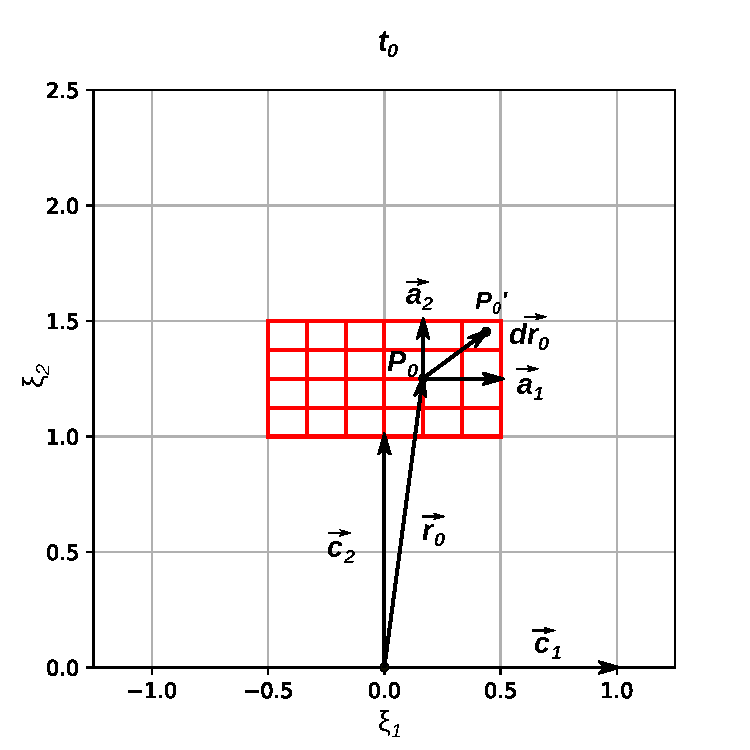
\includegraphics[width=4.5cm]{../img/state_0_00.pdf}~
	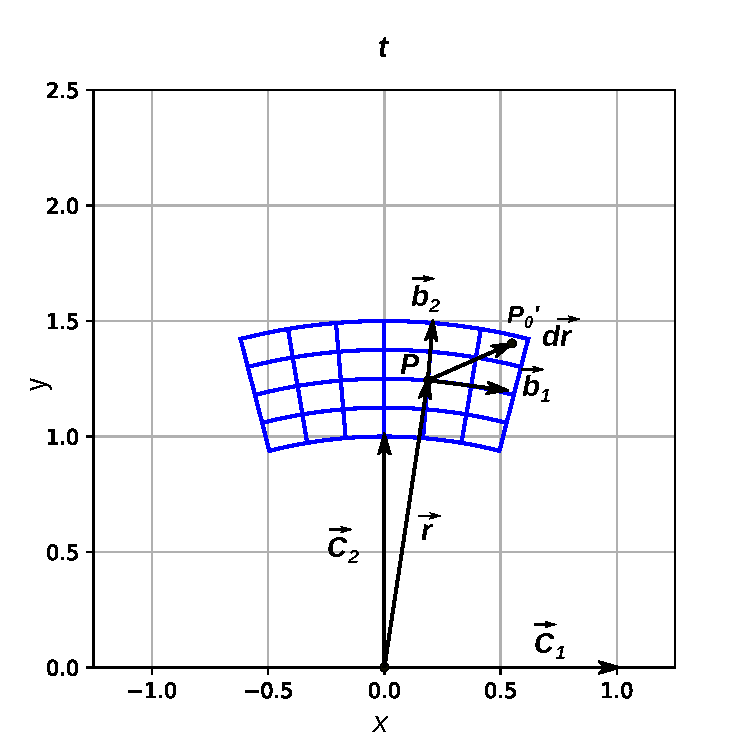
\includegraphics[width=4.5cm]{../img/state_0_50.pdf}	
	

\begin{exampleblock}{Определение}
	\parbox{\textwidth}{
			\centering
		\begin{tabular}{p{5cm}|p{5cm}}
		Лагранжев тензор деформации в представлении Грина & Эйлеров тензор деформации в представлении Альманси \\
		\hline
		$E_0 = \varepsilon_{ij} \vec{a}^i\vec{a}^j$ & $E = \varepsilon_{ij} \vec{b}^i\vec{b}^j$
		\end{tabular}
		
		
		\medskip 
		Здесь $ 2\varepsilon_{ij}= g_{ij}-h_{ij} =\vec{b}_i\cdot\vec{b}_j - \vec{a}_i\cdot\vec{a}_j$.	
	}
\end{exampleblock}




}


\frame{
	\frametitle{ Перемещение }
	
	\centering
	
	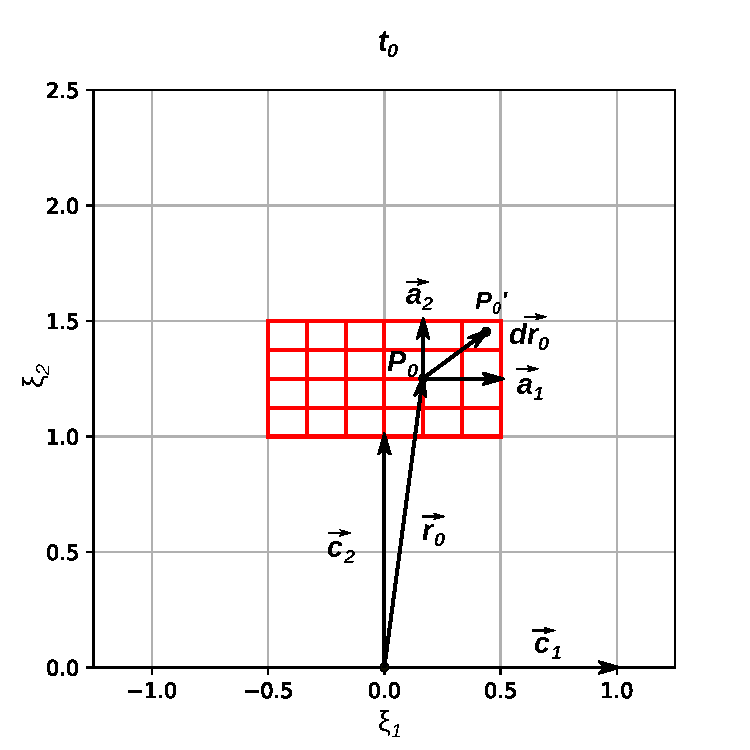
\includegraphics[width=5cm]{../img/state_0_00.pdf}~
	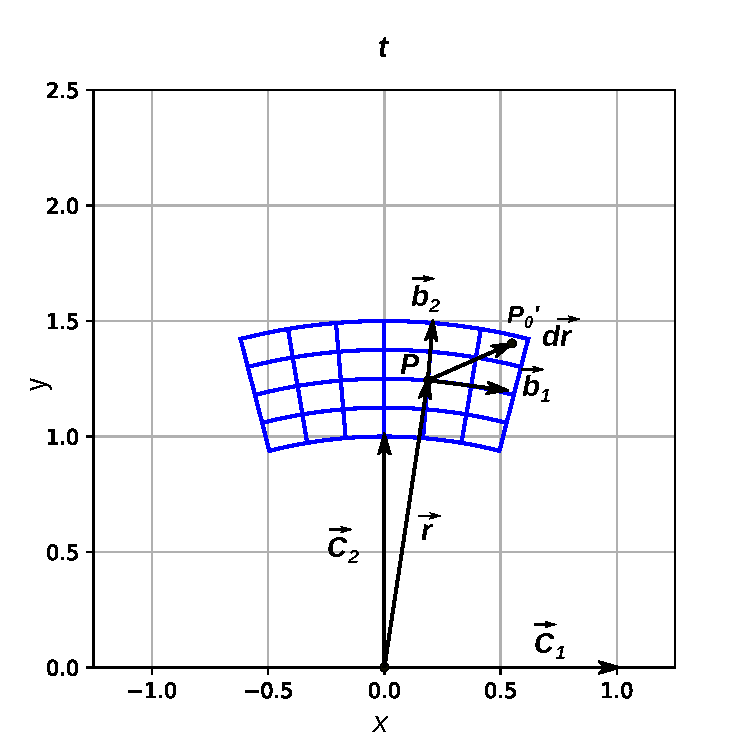
\includegraphics[width=5cm]{../img/state_0_50.pdf}
	
	\begin{exampleblock}{Определение}
		\parbox{\textwidth}{
			Введём вектор перемещения жидкой частицы $\vec{w}$  по следующей формуле
			\[
				\vec{w} = \vec{r}-\vec{r}_0
			\]
			
		}
	\end{exampleblock}
}

\frame{
	\frametitle{ Связь метрического тензора и вектора перемещения }
	
	\begin{exampleblock}{Соглашение}
		\parbox{\textwidth}{
			Пусть в базисе $\vec{a}_j$ разложение $\vec{w}$ будет обозначаться через $u^j$, а в базисе $\vec{b}_i$ через $w^i$
			\[
			\vec{w} = u^j \vec{a}_j= w^i \vec{b}_i
			\]
			
		}
	\end{exampleblock}\pause
	
	\parbox{\textwidth}{
		Используя определение вектора перемещения,
		\[
		\pd{\vec{w}}{\xi^i} =  \pd{\vec{r}}{\xi^i} - \pd{\vec{r}_0}{\xi^i} = \vec{b}_i - 	\vec{a}_i  \, \Rightarrow \, 
		\left|
		\begin{array}{l}
		\vec{a}_i = \vec{b}_i - \displaystyle\pd{\vec{w}}{\xi^i},\\
		\vec{b}_i = \vec{a}_i + \displaystyle\pd{\vec{w}}{\xi^i}.
		\end{array}\right.
		\]\pause Отсюда
		\begin{eqnarray*}
		g_{ij} & = & \vec{b}_i\cdot\vec{b}_j = \vec{a}_i\cdot\vec{a}_j +\vec{a}_i\cdot\pd{\vec{w}}{\xi^j} + \vec{a}_j\cdot\pd{\vec{w}}{\xi^i}+
		\pd{\vec{w}}{\xi^i}\cdot\pd{\vec{w}}{\xi^j},\\
		h_{ij} & = & \vec{a}_i\cdot\vec{a}_j  =  \vec{b}_i\cdot\vec{b}_j - \vec{b}_i\cdot\pd{\vec{w}}{\xi^j} - \vec{b}_j\cdot\pd{\vec{w}}{\xi^i}+
		\pd{\vec{w}}{\xi^i}\cdot\pd{\vec{w}}{\xi^j}.\\ 
		\end{eqnarray*}
		
%		Отсюда из определения тензора деформаций и формулы производной от перемещения
%		\[
%		g_{ij}-h_{ij} = \pd{\vec{w}}{\xi^i} \cdot \pd{\vec{w}}{\xi^j} + \vec{a}_i\cdot\pd{\vec{w}}{\xi^j} + \vec{a}_j\cdot\pd{\vec{w}}{\xi^i} = 2 \varepsilon_{ij}.
%		\]
	}
	
}

\frame{
	\frametitle{ Производная от координатных линий }
	
	\parbox{\textwidth}{
		Рассмотрим	
		\[
		\pd{\vec{w}}{\xi^i} = \pd{}{\xi^i} \left( u^j\vec{a}_j \right) = \pd{u^j}{\xi^i}\vec{a}_j + u^j \pd{\vec{a}_j}{\xi^i} = \left( \pd{u^k}{\xi^i} + u^j \Gamma_{ji}^{0k}\right)\vec{a}_k,
		\]
		\[
		\pd{\vec{w}}{\xi^i} = \pd{}{\xi^i} \left( w^j\vec{b}_j \right) = \pd{w^j}{\xi^i}\vec{b}_j + w^j \pd{\vec{b}_j}{\xi^i} = \left( \pd{w^k}{\xi^i} + w^j \Gamma_{ji}^{k}\right)\vec{b}_k.
		\]
	}
	\begin{exampleblock}{Определение}
		\parbox{\textwidth}{
			Символы $\Gamma_{ji}^{k}$ и $\Gamma_{ji}^{0k}$, имеющие следующие определения
			\[
				\pd{\vec{a}_k}{\xi^i} = \Gamma_{ki}^{0j}\vec{a}_j,\quad
				\pd{\vec{b}_k}{\xi^i} = \Gamma_{ki}^{j}\vec{b}_j,
			\]
			называются \alert{символами Кристофеля} и характеризуют искривление пространства. Они \alert{не являются} тензорами и тождественно равны $0$ для абсолютной декартовой системы координат $\vec{c}_l$.
		}
	\end{exampleblock}


}


\frame{
	\frametitle{ Выражение тензора деформации через вектор перемещения }
	\parbox{\textwidth}{
		Таким образом, имеем
		\[
		\varepsilon_{ij} = \frac{1}{2}
		\left(
		\vec{a}_i\cdot\pd{\vec{w}}{\xi^j}+\vec{a}_j\cdot\pd{\vec{w}}{\xi^i}+\pd{\vec{w}}{\xi^i}\cdot\pd{\vec{w}}{\xi^j}
		\right)
		=
		\]
		\[
		=\frac{1}{2}
		\left(
		\vec{b}_i\cdot\pd{\vec{w}}{\xi^j}+\vec{b}_j\cdot\pd{\vec{w}}{\xi^i}-\pd{\vec{w}}{\xi^i}\cdot\pd{\vec{w}}{\xi^j}
		\right).
		\]\pause
		
		Для бесконечно малых деформаций, пренебрегают членами второго порядка, тогда
		\[	
		\varepsilon_{ij} \approx \frac{1}{2}
		\left(
		\vec{a}_i\cdot\pd{\vec{w}}{\xi^j}+\vec{a}_j\cdot\pd{\vec{w}}{\xi^i}
		\right) \,\text{или}\,
%		\]
%		\[
		\varepsilon_{ij} \approx \frac{1}{2}
		\left(
		\vec{b}_i\cdot\pd{\vec{w}}{\xi^j}+\vec{b}_j\cdot\pd{\vec{w}}{\xi^i}
		\right).
		\]
		В этом случае $\varepsilon_{ij}$ называют \alert{тензором малых деформаций}.
	}
	
}

\frame{
	\frametitle{ Тензор скоростей деформаций }
	
	\begin{exampleblock}{Определение}
		\parbox{\textwidth}{
			Рассмотрим тензоры деформаций $\varepsilon_{ij}$ и $\varepsilon_{ij}'$ в два близких момента времени $t \geq t_0$ и $t'=t+\Delta t$:
			\[
			\varepsilon_{ij}=\frac{1}{2}(g_{ij} - h_{ij}),\quad
			\varepsilon_{ij}'=\frac{1}{2}(g_{ij}' - h_{ij}),\quad
			\]
			где $g_{ij}$, $g_{ij}'$, $h_{ij}$ -- метрические тензоры в моменты времени $t$, $t'$ и $t_0$.
			
			Назовём \alert{тензором скоростей деформации} величины
			\[
			e_{ij} = \lim_{\Delta t \to 0}\frac{\varepsilon_{ij}'-\varepsilon_{ij}}{\Delta t}= \lim_{\Delta t \to 0}\frac{g_{ij}'-g_{ij}}{\Delta t}.
			\]
		}
	\end{exampleblock}

	\begin{exampleblock}{Свойство}
		\parbox{\textwidth}{
			Величины $e_{ij}$ образуют симметричный ковариантный тензор 2-ого ранга.
			
		}
	\end{exampleblock}
	
}

\frame{
	\frametitle{ Связь между вектором скорости и тензором скоростей деформации }
	
	\parbox{\textwidth}{
		Введём вектор $\Delta\vec{w}$ как перемещение жидкой частицы между временем $t$ и $t'=t+\Delta t$:
		\[
		\Delta\vec{w} = \vec{r}-\vec{r}'.
		\]
		Используя преобразования, полученные ранее, для вектора перемещений имеем
		\[
		\Delta \varepsilon_{ij} = \varepsilon_{ij}'-\varepsilon_{ij} = \frac{g_{ij}'-g_{ij}}{2}=
		\frac{1}{2}\left( \vec{a}_i\cdot\pd{\Delta\vec{w}}{\xi^j}+\vec{a}_j\cdot\pd{\Delta\vec{w}}{\xi^i}+\pd{\Delta\vec{w}}{\xi^i}\cdot\pd{\Delta\vec{w}}{\xi^j}
		\right),
		\]
		где \alert{$\vec{a}_i$ -- сопутствующий базис} в момент времени $t$. Тогда 
		\[
		\lim_{\Delta t \to 0} \frac{\Delta\varepsilon_{ij}}{\Delta t} = \frac{1}{2}
		\left(
		\vec{a}_i\cdot\pd{\vec{v}}{\xi^j}+\vec{a}_j\cdot\pd{\vec{v}}{\xi^i}
		\right), 
		\]
		где $\vec{v}=v^k\vec{a}_k = \lim\limits_{\Delta t \to 0} \Delta \vec{w} /\Delta t$ -- вектор скорости жидкой частицы.
	}
	
}

\frame{
	\frametitle{ Компоненты тензора скоростей деформации в абсолютной системе координат }
		\centering
	
	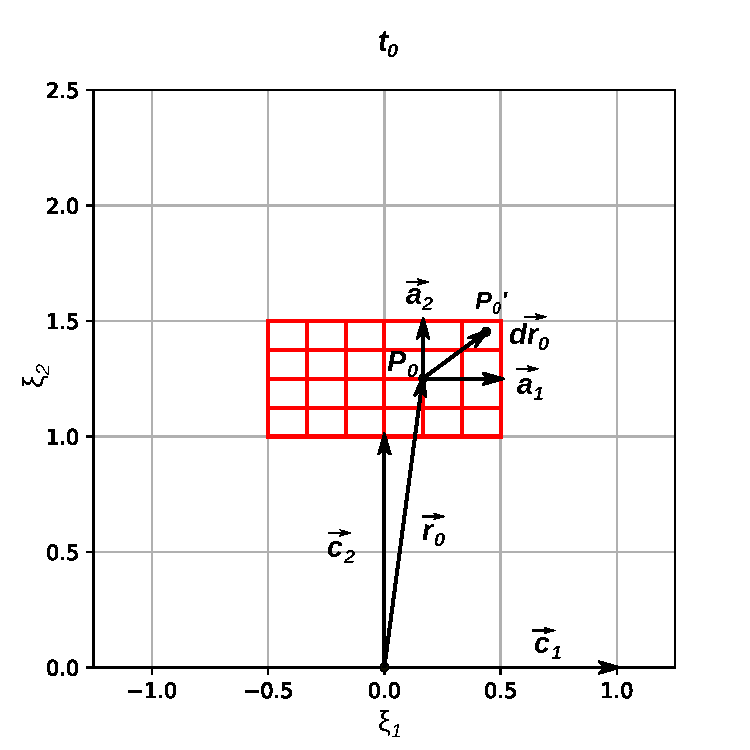
\includegraphics[width=4.5cm]{../img/state_0_00.pdf}
%	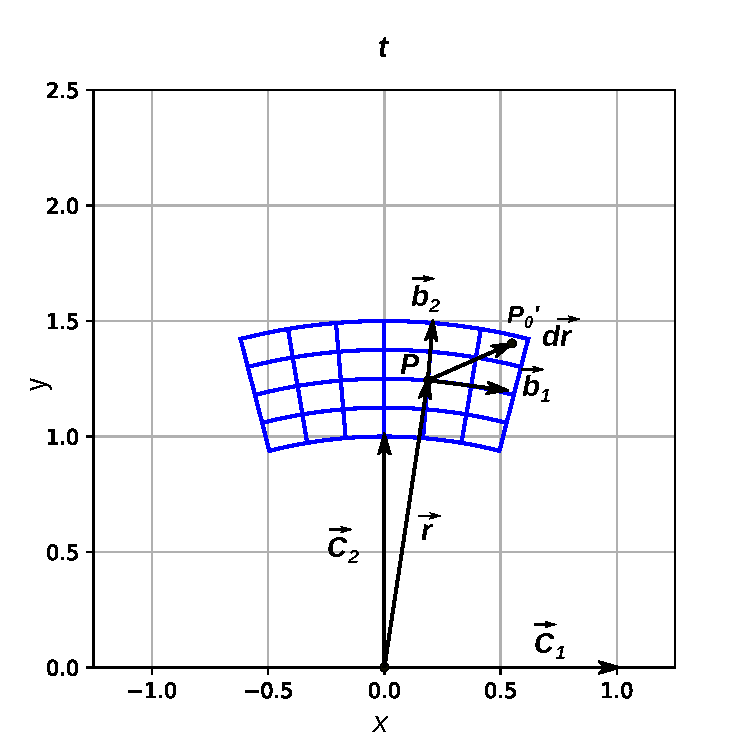
\includegraphics[width=4.5cm]{../img/state_0_50.pdf}	
	
	\parbox{\textwidth}{
%		Компоненты тензора скоростей деформации в абсолютной декартовой системе координат $\vec{c}_i$ в силу тензорной природы имеют вид 
		\[
		\bar{e}_{ij} = e_{kl} \pd{\xi^k}{x^i} \pd{\xi^l}{x^j},
		\]
		где $\bar{e}_{kl}$, $e_{kl}$ -- компоненты в абсолютной декартовой $\vec{c}_i$ и сопутствующей криволинейной системах координат тензора скоростей деформации; $\xi_i=\xi_i\argtx$ -- обратное преобразование
		 %\alert{(не обязательно является траекторией движения)
		 }.
		


}
	



\frame{
	\frametitle{ Компоненты тензора скоростей деформации в абсолютной системе координат }

		Пусть разложение сопутствующего базиса и вектора скорости в абсолютной системе координат имеют вид 
		\[
		\vec{a}_i = \pd{\vec{r}}{\xi_i}=\displaystyle\pd{x^k}{\xi_i}\vec{c}_k,\quad
		\vec{v}=v^r\vec{c}_r.
		\]\pause
%	\medskip
		Рассмотрим, как преобразуется при переходе к абсолютной декартовой системе координат слагаемое вида $\displaystyle\vec{a}_i\cdot\pd{\vec{v}}{\xi_j}$:
		\[
		\left(\vec{a}_i\cdot\pd{\vec{v}}{\xi_j}\right) \pd{\xi^i}{x^p} \pd{\xi^j}{x^q}=
		\left(\pd{x^k}{\xi_i}\vec{c}_k\right)\cdot 
		\left(\pd{v^r}{x^l}\pd{x^l}{\xi^j}\vec{c}_r\right) \pd{\xi^i}{x^p} \pd{\xi^j}{x^q}=
		\]
		\[
		=
		\left(\pd{x^k}{\xi_i} 
		\pd{v^r}{x^l}\pd{x^l}{\xi^j} \delta^k_r \right) \pd{\xi^i}{x^p} \pd{\xi^j}{x^q}
		=
		\pd{x^k}{\xi_i}
		\pd{x^l}{\xi^j} \pd{\xi^i}{x^p} \pd{\xi^j}{x^q} \pd{v^k}{x^l} = 
		\delta_k^p\delta^l_q\pd{v^k}{x^l}		
		=
		\pd{v^p}{x^q}.
		\]
}


\frame{
	\frametitle{  Компоненты тензора скоростей деформации в абсолютной системе координат }
	
	\begin{exampleblock}{Результат}
	\parbox{\textwidth}{
	Используя полученное выражение, компоненты тензора скоростей деформации в абсолютной декартовой системе координат имеют вид
	\[
	e_{ij} = \frac{1}{2}\left( \pd{v^i}{x^j} + \pd{v^j}{x^i}\right).
	\]
}	\end{exampleblock}\pause


	\begin{exampleblock}{Свойства}
		\parbox{\textwidth}{
			\begin{itemize}
				\item Симметричность $e_{ij}=e_{ji}$
				\item Характеризует состояние среды в данный момент времени в отличие от тензора деформации
				\item $e_{ij} \Delta t = \varepsilon_{ij}$ -- являются компонентами тензора малых деформаций
			\end{itemize}

			
		}
	\end{exampleblock}
	
}

\frame{
	\frametitle{ Распределение скоростей в бесконечно малой частице  }
	\centering
	
	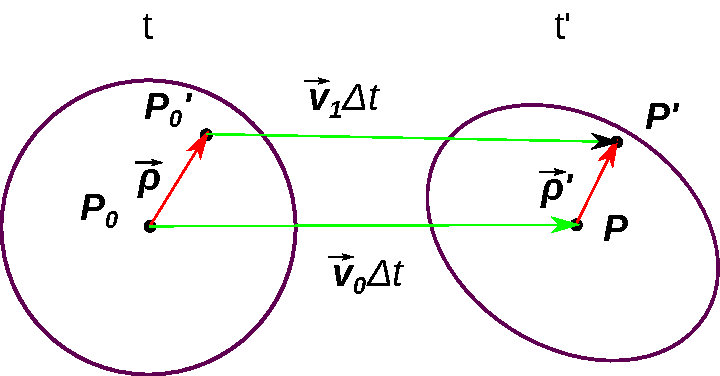
\includegraphics[width=5cm]{../img/velocity_of_small_volume.pdf}

	\begin{exampleblock}{Постановка задачи}
		\parbox{\textwidth}{
			Рассмотрим окрестность точки $P_0$ с лагранжевыми координатами $\xi_i$ и точку из окрестности $P_0'$ с лагранжевыми координатами $\xi_i+d\xi_i$. За время $\Delta t$ точки $P_0$ и $P_0'$, образующие вектор $\vec{\rho}$, перейдут в точки $P$, $P'$, образующие вектор $\vec{\rho}'$.
			
			\bigskip
			Требуется связать изменения вектора $\vec{\rho}$ с тензором скоростей деформаций. Рассмотрение ведется в абсолютной декартовой системе координат.
			
		}
	\end{exampleblock}

}


\frame{
	\frametitle{ Соотношения для изменения вектора направления в окрестности выбранной точки }

	\centering

	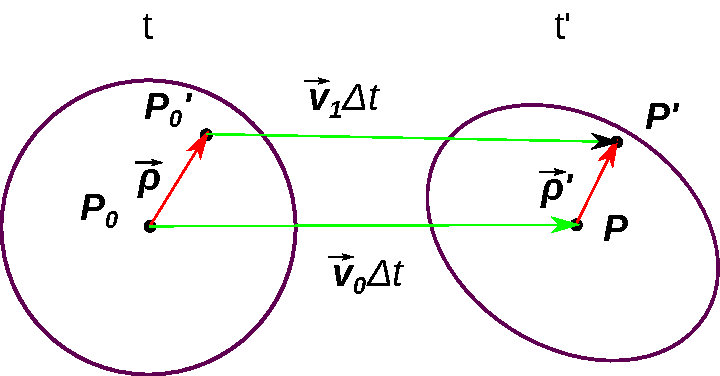
\includegraphics[width=5cm]{../img/velocity_of_small_volume.pdf}

	\bigskip
	\parbox{\textwidth}{
	Из рисунка видно, что с точностью до первого порядка по $\Delta t$
	\[
	\vec{\rho}'=\vec{\rho}+(\vec{v}_1-\vec{v}_0)\Delta t,
	\]
	где $\vec{v}_1$, $\vec{v}_2$ -- скорости движения точки $P_0$ в $P$ и $P_0'$ в $P'$ за малое время  $\Delta t$.
	}
}

\frame{
	\frametitle{ Соотношения для изменения вектора направления в окрестности выбранной точки   }

	\centering
	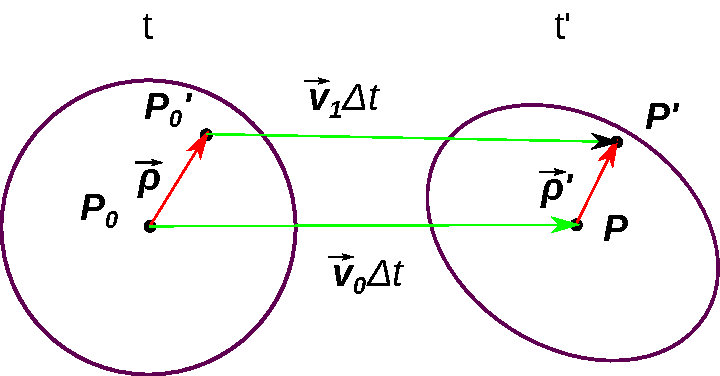
\includegraphics[width=5cm]{../img/velocity_of_small_volume.pdf}	
	
	\bigskip
	\parbox{\textwidth}{
		
		При разложении Тейлора для вектора скорости в окрестности точки $P_0$ имеем
	 	\begin{equation}
	 	\label{eq:rho_transform}
		\vec{v}_1=\vec{v}_0+\left.\left(\pd{\vec{v}}{\xi^i}\right)\right|_{P_0} \rho^i + \vec{\rho}O(\rho).
		\end{equation}
		
		
	}
	
}


\frame{
	\frametitle{ Соотношения для изменения вектора направления в окрестности выбранной точки }

\begin{exampleblock}{}
	\parbox{\textwidth}{
		
		Подставляя соотношение для скорости в соотношение для изменения длины получим		
		\[
		\vec{\rho}'=\vec{\rho}+\left.\left(\pd{\vec{v}}{\xi^i}\right)\right|_{P_0}\rho^i\Delta t + \vec{\rho}O(\rho\Delta t )
		\]
		
		\bigskip
		Из этого соотношения видно, что бесконечно малая жидкая частица за время $\Delta t$ претерпевает бесконечно малое аффинное преобразование с точностью до $\vec{\rho}O(\rho\Delta t)$.
	}
\end{exampleblock}
	
}

\frame{
	\frametitle{ Разложение скорости в окрестности выбранной точки }
	
	\begin{exampleblock}{Разложение}
		\parbox{\textwidth}{
			Используя теорему о разложении тензора на симметричный и антисимметричный тензор представим $\vec{v}_1$ в виде
			\[
			\vec{v}_1=\vec{v}_0+\left.\left(\pd{\vec{v}}{\xi^i}\right)\right|_{P_0} \rho^i + \vec{\rho}O(\rho)=
			\]
			\[
			=
			\vec{v}_0+\frac{1}{2}\left(\pd{v^i}{\xi^k}+\pd{v^k}{\xi^i}\right)\rho^i\vec{c}_k+
			\frac{1}{2}\left(\pd{v^k}{\xi^i}-\pd{v^i}{\xi^k}\right)\rho^i \vec{c}_k+ \vec{\rho}O(\rho)=
			\]
			\[
			=
			\vec{v}_0+e_{ik}\rho^i \vec{c}_k+\omega_{ki}\rho^i \vec{c}_k+ \vec{\rho}O(\rho),
			\]
			где $e_{ik}$ -- компоненты симметричного тензора скоростей деформации, а
			\[
				\omega_{ki}=\frac{1}{2}\left(\pd{v^k}{\xi^i}-\pd{v^i}{\xi^k}\right)
			\]
			компоненты антисимметричного тензора.
			
		}
	\end{exampleblock}
}

\frame{
	\frametitle{ Разложение скорости на составляющие }
	
	\begin{exampleblock}{Теорема Коши-Гельмгольца }
		\parbox{\textwidth}{
			Рассмотрим декартову систему координат, так что
			\[
			\vec{\rho}=x^1\vec{c}_1+x^2\vec{c}_2+x^3\vec{c}_3,
			\]
			тогда
			\[
				\vec{v}_1 = \vec{v}_0 + \vec{\omega} \times \vec{\rho} + \operatorname{grad} \Phi +\vec{\rho}O(\rho),			
			\]
%			где
			\[
			\Phi = \frac{1}{2}e_{pq} x^p x^q,\quad
			\vec{\omega} = \omega^i\vec{c}_i=\frac{1}{2}
			\left|
			\begin{array}{ccc}
			\vec{c}_1 & \vec{c}_2 & \vec{c}_3 \\
			\displaystyle\pd{}{x^1} & \displaystyle\pd{}{x^2} & \displaystyle\pd{}{x^3}\\
			v_1^1 & v_1^2 & v_1^3
			\end{array}
			\right|=
			\frac{1}{2}\operatorname{rot}\vec{v}.
			\]
			Сравнивая это выражение с формулой для скорости движения абсолютно твёрдого тела имеем, скорость жидкой частицы складывается из \alert{скорости поступательного движения, вращательного и скорости чистой деформации}.
		}
	\end{exampleblock}
}

\frame{
	\frametitle{ Скорость относительного удлинения }
	
	\begin{exampleblock}{}
		\parbox{\textwidth}{
			Рассмотрим относительное удлинение $e_\rho$ вектора $\vec{\rho}$:
			\[
			e_\rho = \frac{1}{|\vec{\rho}|}\frac{d|\vec{\rho}|}{dt}=
			\frac{1}{\rho}\frac{d\rho}{dt}=
			\frac{1}{2}\frac{1}{\rho^2}\frac{d\rho^2}{dt}=
			\frac{1}{2}\frac{1}{\rho^2}\frac{d(\vec{\rho}\cdot\vec{\rho})}{dt}=
			\frac{1}{\rho^2}\left(\vec{\rho}\cdot\frac{d\vec{\rho}}{dt}\right).
			\]\pause			
			Используя разложение из теоремы Коши-Гельмгольца, соотношение (\ref{eq:rho_transform}) при $\Delta t \to 0$ и то, что $\vec{\rho}\cdot(\vec{\omega}\times\vec{\rho})=0$, получим
			\[
			e_{\rho}=\frac{1}{\rho^2}\left(\vec{\rho}\cdot\frac{d\vec{\rho}}{dt}\right)=
			\frac{1}{\rho^2}\left(\vec{\rho}\cdot \operatorname{grad}\Phi \right)=
			\frac{1}{\rho^2}\left(\pd{\Phi}{x^1} x^1+\pd{\Phi}{x^2} x^2 + \pd{\Phi}{x^3} x^3\right)=
			\]
			\[
			=\frac{2\Phi}{\rho^2}=e_{ij}\frac{x^i}{\rho}\frac{x^j}{\rho}=e_{ij}\alpha^i\alpha^j,
			\]
			где $\alpha^i=\displaystyle\frac{x^i}{\rho}=\cos(\rho,x^i)$.
			
		}
	\end{exampleblock}
}

\frame{
	\frametitle{  Скорость относительного удлинения }
	
	\begin{exampleblock}{Вывод}
		\parbox{\textwidth}{
			Скорость относительного удлинения задаётся квадратичной формой
			\[
			e_\rho = e_{ij}\alpha^i\alpha^j,
			\]
			где $\alpha^i=\displaystyle\frac{x^i}{\rho}=\cos(\rho,x^i)$, $e_{ij}$ -- компоненты тензора скоростей деформации.
			
			\medskip
			Компоненты тензора скоростей деформации с одноимёнными индексами являются скоростями относительных удлинений отрезков среды, первоначально направленных параллельно соответствующим координатным осям. 
			
		}
	\end{exampleblock}
	
}

\frame{
	\frametitle{ Скорость относительного удлинения  }
	
	\begin{exampleblock}{Вывод}
		\parbox{\textwidth}{
		Вспомнив, что 
		\[
		\varepsilon_{ij}=e_{ij}\Delta t,
		\]
		где $\varepsilon_{ij}$ -- тензор малых деформаций, получим свойство недиагональных элементов тензора скоростей деформаций.
		Так как
		\[
		\sin\alpha_{ij}=2\varepsilon_{ij},
		\]
		где $\alpha_{ij}$ -- угол скашивания изначально прямого угла,
		то недиагональные компоненты тензора $e_{ij}$ $i \neq j$ равны половине скорости скашивания первоначально прямых углов, образованных отрезками среды, в данный момент времени параллельными соответствующим координатным осям.
		}
	\end{exampleblock}
}


\frame{
	\frametitle{ Главные оси и главные значения тензора скоростей деформаций}
	\parbox{\textwidth}{
	Квадратичная форма 
	\[
	e_\rho = e_{ij} \alpha^i \alpha^j,
	\]
	где $\alpha^i=\cos(\rho,x^i)$, аналогично, как в случае с тензором деформации, анализируется на экстремальные значения на единичной сфере. \pause 
	}
	

	\begin{exampleblock}{Вывод}
		\parbox{\textwidth}{
			Максимальные скорости относительного удлинения совпадают с главными значениями тензора скоростей деформации $e_1$, $e_2$, $e_3$, а направления, на которых они реализуются совпадают с собственными векторами тензора скоростей деформации. Очевидно, что если $e_i > 0$, то имеет место растяжение, а если $e_i < 0$, то сжатие.
			
		}
	\end{exampleblock}
	
}


\frame{
	\frametitle{ Литература }
	\begin{itemize}[partopsep=1pt,label=\textbullet]
		\item  {\em Седов~Л.~И.} Механика сплошной среды. Том 1. М.:Наука, 1970.
		\item {\em Сокольников~И.~С.} Тензорный анализ (теория и применение в геометрии и в механике сплошных сред).  Перевод с англ. Главная редакция физ.-мат. лит. Изд. М.: Наука, 1971.		
	\end{itemize}
	
}

\end{document}